\documentclass[a4paper,11pt]{article}
\usepackage[margin=.8in]{geometry}
\usepackage[utf8]{inputenc}

\usepackage{listings}
\usepackage{amsfonts}
\usepackage{amsmath}
\usepackage{amsthm}
\usepackage{hyperref}
\hypersetup{
    colorlinks=true,
    linkcolor=magenta
}
\usepackage{graphicx}


\title{Exercise 4}
\author{Deep Learning Lab}

\begin{document}

\maketitle

\section{MNIST Digit Classification Using Feed-Forward Neural Networks}
Using the code presented in the lecture (at the end of Sec.\,2.2, ``Put them all together") as a starting point, in this task, you will build a digit classification system using feed-forward neural networks.
\begin{enumerate}
\item The validation set was missing in the code presented in the lecture.
Create a validation set by using the first 55000 samples of the original training data for training and the rest for validation.
Hint: Use \texttt{torch.utils.data.SubsetRandomSampler} and \texttt{sampler} option of \texttt{torch.utils.data.DataLoader}.
 \item Add the necessary lines of code to monitor the training progress (i.e.~training and validation losses).
Remember, you should only look at training and validation losses during training!
\item Make sure that your code works with the points above.
Now try to find a better set of hyper-parameters.
You may try different learning rates, batch sizes, number of epochs,
sizes of hidden layers, number of hidden layers,
activation functions,
and optimization algorithm. 
\item Once you settle on a final model, compute the test set accuracy.
\end{enumerate}

\section{Binary Classification}

\begin{enumerate}

 \item Consider the following function that creates a classification dataset where observations are drawn from multivariate Gaussian distributions:
 
  \begin{lstlisting}[language=Python, frame=tb, caption=Multivariate Gaussians dataset.]

def create_dataset(means, std, sample_size, seed=None):
    random_state = np.random.RandomState(seed)

    X = np.zeros((sample_size, len(means[0])), dtype=np.float32)
    Y = np.zeros((sample_size, len(means)), dtype=np.float32)

    cov = np.eye(len(means[0]))*(std**2)

    for i in range(sample_size):
        c = random_state.randint(len(means))
        X[i] = random_state.multivariate_normal(means[c], cov)
        Y[i, c] = 1.

    return X, Y
  \end{lstlisting}
  
  \begin{enumerate}
    \item Using this function, create a dataset with two classes. Place one mean at $(-1, 1)$ and another at $(1, -1)$. Let the standard variation be $0.5$, the sample size $500$, and the seed $0$.
    \item Use \href{https://matplotlib.org/3.1.1/gallery/shapes_and_collections/scatter.html}{plt.scatter} to plot the observations in your dataset, coloring the points according to their classes. Tip: use the colors $0$ and $1$ to represent the classes, and set the colormap (cmap) to \emph{plt.cm.RdBu}.
    \item Train a multilayer perceptron using your dataset.
    \item Use your multilayer perceptron to predict the class of observations in a grid on the set $[-3, 3] \times [-3, 3]$. Visualize the decision boundary by creating a contour plot based on these predictions (see Fig. \ref{fig:decision}). Tip: use np.meshgrid to create a grid of observations and plt.contourf to create the contour plot. \href{http://scikit-learn.org/stable/auto_examples/classification/plot_classifier_comparison.html}{Here} is an example.
    \item Observe the consequences of changing the parameters that you used to create your dataset (means, standard deviation, sample size).
    \item Observe the consequences of changing model hyperparameters.

  \begin{figure}[h]
  \caption{Example decision boundary.}
  \label{fig:decision}
  \centering
    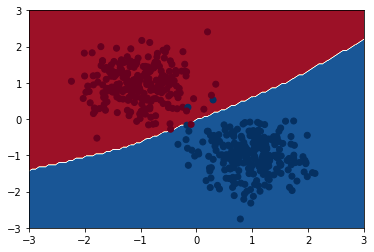
\includegraphics[width=0.5\textwidth]{figures/decision.png}
    \end{figure}

\item Do the same on the following dataset:
  \begin{lstlisting}[language=Python, frame=tb, caption=Generate ``moon''-form datapoints.]
from sklearn.datasets import make_moons

X, y = make_moons(n_samples=500, noise=0.2)
plt.scatter(X[:, 0], X[:, 1], c=y, cmap=plt.cm.RdBu)
  \end{lstlisting}

\begin{figure}[h]
\caption{Dataset with two moons.}
\label{fig:decision}
\centering
  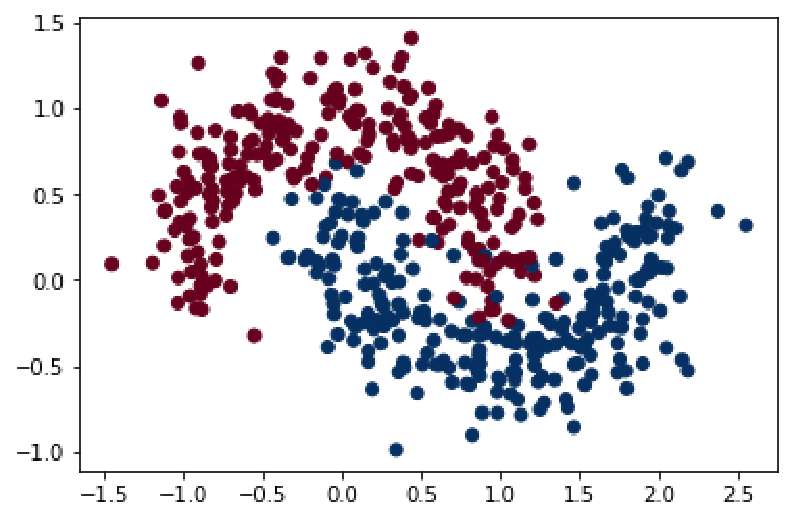
\includegraphics[width=0.5\textwidth]{figures/moon.pdf}
  \end{figure}


  \end{enumerate}
  
  
%  \begin{figure}[h]
%  \caption{Example decision boundary.}
%  \label{fig:decision}
%  \centering
%    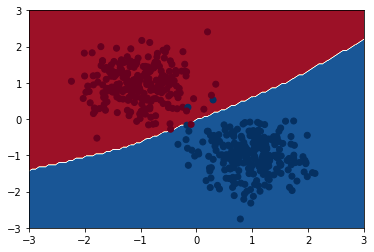
\includegraphics[width=0.5\textwidth]{figures/decision.png}
%    \end{figure}



\end{enumerate}


\end{document}
